\section{Concept}

This section illustrates the concrete idea that we have now synthesized from our general suggestions.
It is no way complete or final.
As most of these concepts are based on the location sharing, we propose to implement the location sharing first and then expand the other concepts on top of that.

\subsection{Location Sharing}
\label{location_sharing}

todo

\subsection{Video Sharing}

todo

\subsection{Screencast Sharing}

todo

\subsection{Calendar Sharing}

todo

\subsection{Data to Go}
\label{data2go}

One part of the proposed architecture would be location aware data sharing within the display network.
This is envisioned to work in two general modes, which are based on the underlying location sharing described in section \ref{location_sharing}.
The first would allow the pinning of data to a user's location, leaving its visibility set to private.
This would allow a user to take data with him when going to a colleagues' office for a meeting.
Apart from making the data available to the system, no further care would need to be taken to keep data readily available.
The second mode would allow data to be shared by sending it to a certain location, for example a meeting room.
This would make the data publicly available, primarily for that location.
Once that shared data is accessed from the location, its ownership would transfer away from its originating owner to a public ownership based on the location.

Figure \ref{data_share_sequence} shows some concepts for how the system would handle the data via the proposed modes.
Private sharing of data is also allowed by pinning data to another person.
This person then has access to the data based on their location, although ownership only transfers at a specific event that will have to be specified based on user preference and usage for download.

\begin{figure}
	\centering
	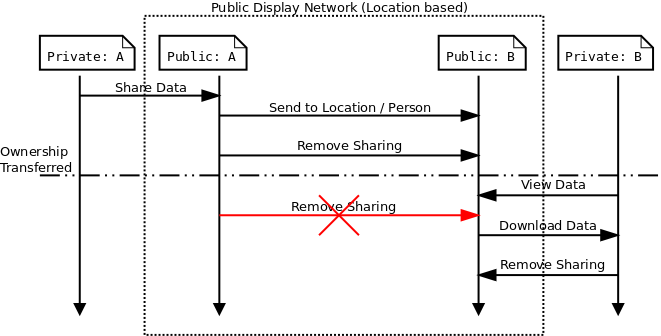
\includegraphics[width=\linewidth]{img/data_sharing.png}
	\caption[Data Sharing Sequence]{Informal sequence diagram of how data sharing might work, including some privacy and security options.}
	\label{data_share_sequence}
\end{figure}

As no data can be generated in the first iterations of the system (although such capabilities might well be added), a way to transfer data to and from the system will be required.
Such a way also makes sense from a user point of view, as the system is to be used alongside a broad range of private computers of the users.
To solve this data transfer gap, we propose a client program for a variety of devices that allows data control.
Pinning data to the user's own location (as in his private space) can be done by simply allowing the user to drag\&drop a file onto the client application, which will handle any conversion and transferring mechanism.
Similarly, retrieving data from a location or private area can be done by selecting the data via the client.
Having a client for not only desktop computers but also for smartphones would enable a broader and more comprehensive usage of the proposed service system.
